\chapter{Comportamiento longitudinal}
\label{ch:longitudinal-model}

El comportamiento longitudinal es un problema de regresión sobre cómo ha de comportarse la aceleración del \ac{dvu} en función de la información existente alrededor.

Por la naturaleza del problema se han seleccionado dos técnicas diferentes para el ajuste del modelo:

\begin{enumerate}
	\item \ac{mlp}. Al ser un problema de regresión, el uso de \acp{mlp} en el comportamiento longitudinal está justificado a ser considerados éstos aproximadores universales~\cite{hornik1991approximation}\sidenote{El \textit{Teorema de aproximación Universal} postula que un \ac{mlp} con al menos una capa oculta es capaz de aproximar cualquier función si dispone de suficientes neuronas en ésta.}
	\item \ac{fcs}. La formulación de este problema se ajusta muy bien al funcionamiento de estos modelos, donde en función de las entradas y de acuerdo a una serie de reglas, el controlador toma una decisión para la salida. Además, los \ac{fcs} tienen la ventaja de que se puede explicar cómo funcionan, cosa que no es posible para un \ac{mlp} con una o más capas ocultas.
\end{enumerate}

Ambos modelos se entrenaran ajustando sus parámetros con un procedimiento basado en el descenso del gradiente denominado ADAM~\cite{kingma2014adam}. Su aplicación a los \ac{mlp} es directa, pero para \acp{fcs} es necesaria una representación que permita el uso de este método para su optimización. Esta representación es una de las aportaciones de esta tesis y se se explica en el apéndice \nameref{ch:fuzzy-controller-adjustment}.

\paragraph{Modelo \ac{fcs}}

Se han tomado las siguientes decisiones de diseño para facilitar el desarrorrollo del controlador. Aún así, éstas son fácilmente modificables:

\begin{itemize}
	\item Las funciones de pertenencia serán, o bien una línea descendente en el caso del primer conjunto difuso de una partición, una línea ascendente en el caso del último o trapecios en el caso del resto.
	\item Las $t$-norma y $t$-conorma serán el máximo y el mínimo respectivamente. La $t$-norma se usará como operador asociado al AND lógico y a la implicación, mientras que la $t$-conorma se usará como operador asociado al OR lógico y a la acumulación.
	\item El controlador será de tipo Sugeno, representando las funciones de salida como conjuntos difusos de tipo singletón y con función de defuzzificación CoGS\sidenote{
		$CoGS = \sum_{i=1}^n w_i \cdot o_i$
	}.
	\item El tamaño de las particiones difusas será dado de antemano.
	\item El controlador tendrá una única variable de salida.
\end{itemize}

\begin{table}[t]
	\caption[Descripción de los conjuntos de datos]{Descripción de los conjuntos de datos para el entrenamiento de los modelos.}
	\label{tbl:adjusted-fcs}
	\begin{tabular}{lllll}
		\toprule
		Nombre & Entradas & Salidas & Tamaño (training) & Tamaño (test) \\
		\midrule
		$LT_{S_1}$ & \yep & \yep & \yep & \\
		$LT_{S_2}$ & \nop & \yep & \yep & \\
		$LT_{S_3}$ & \nop & \yep & \yep & \\
		$LT_{S_A}$ & \nop & \yep & \yep & \\
		$CT_{S_1}$ & \nop & \yep & \yep & \\
		$CT_{S_2}$ & \yep & \nop & \yep & \\
		$CT_{S_3}$ & \yep & \yep & \yep & \\
		$CT_{S_A}$ & \yep & \yep & \yep & \\
		\bottomrule
	\end{tabular}
\end{table}

Cada uno de los controladores se ha entrenado durante XXX epochs. En la Figura~\ref{fig:adjusted-fcs} se puede observar la evolución en general y un detalle de la disminución del error en test de los controladores.

\begin{figure}
	\centering
	\subfloat[]{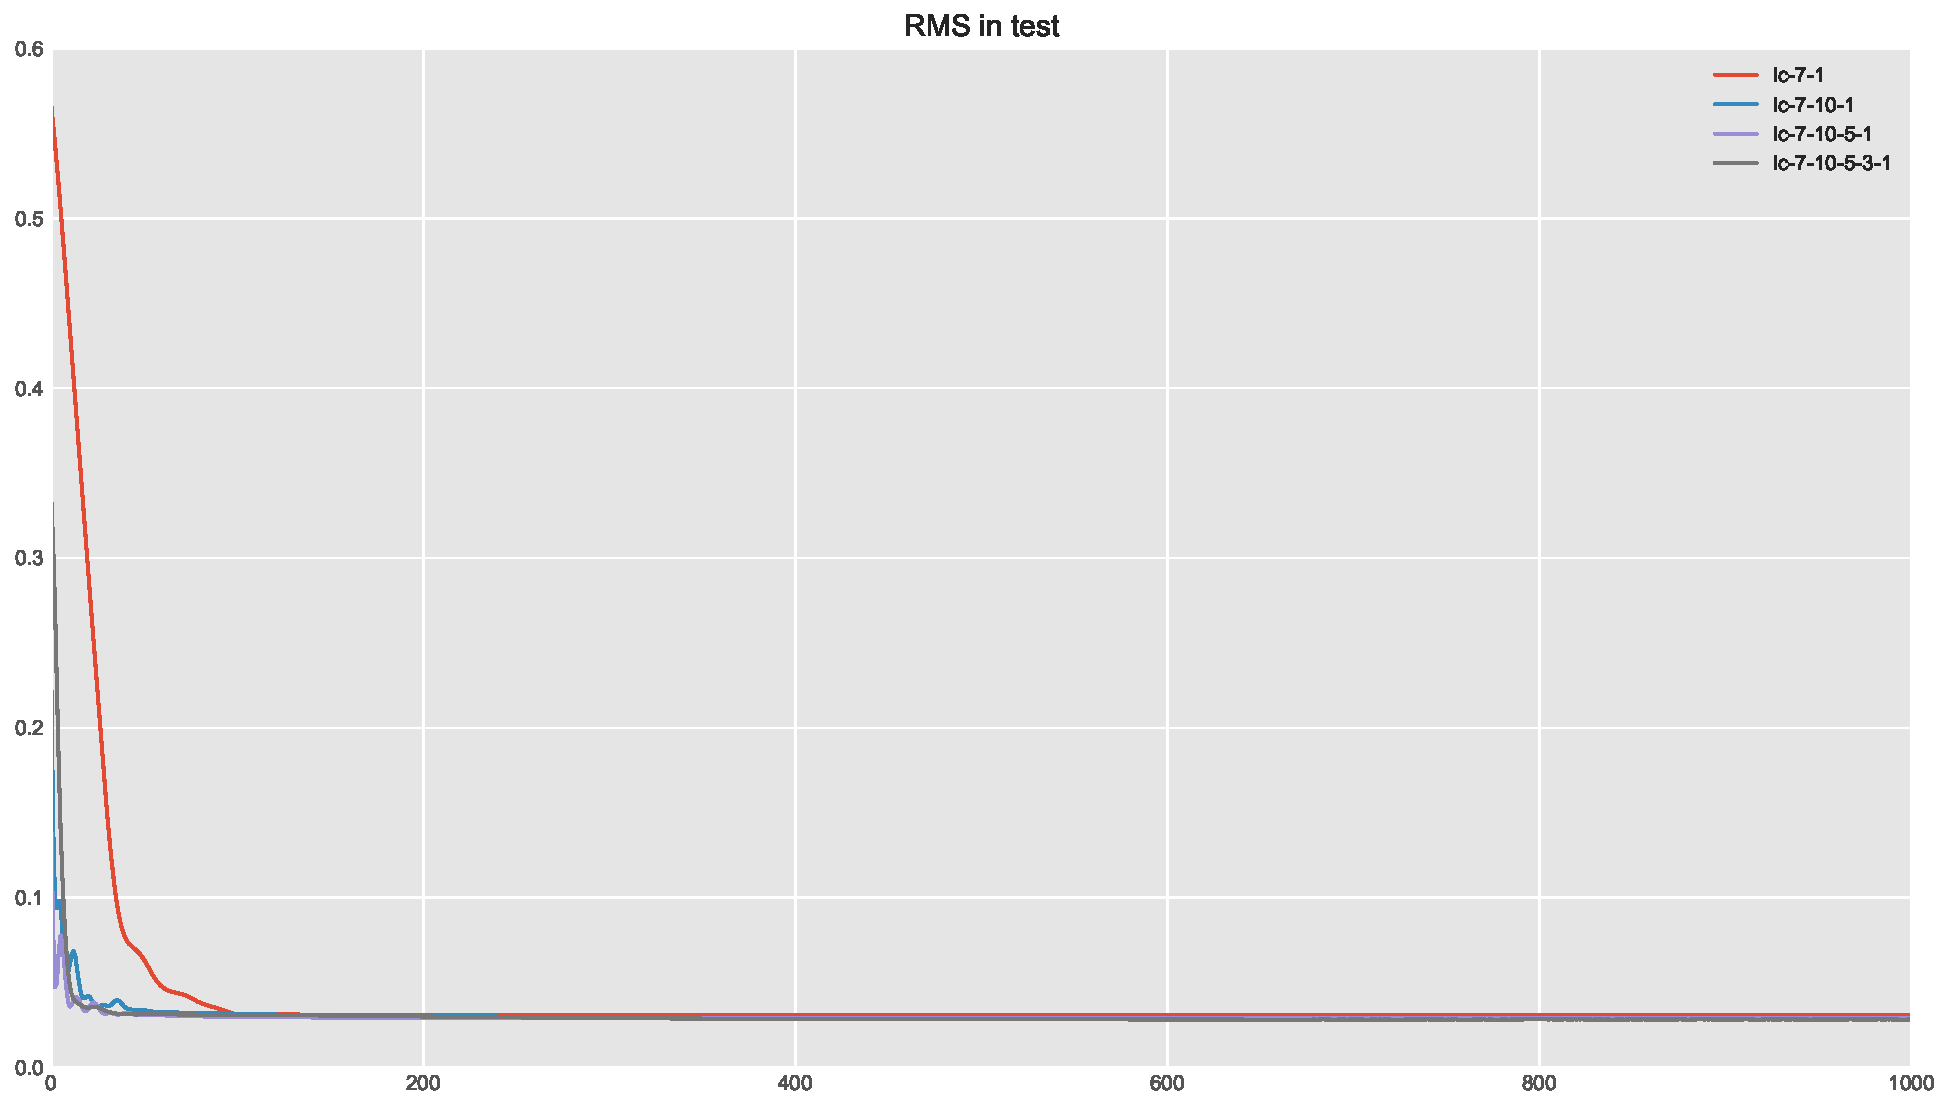
\includegraphics[width=.45\textwidth]{fcs-all-test}}\qquad
	\subfloat[]{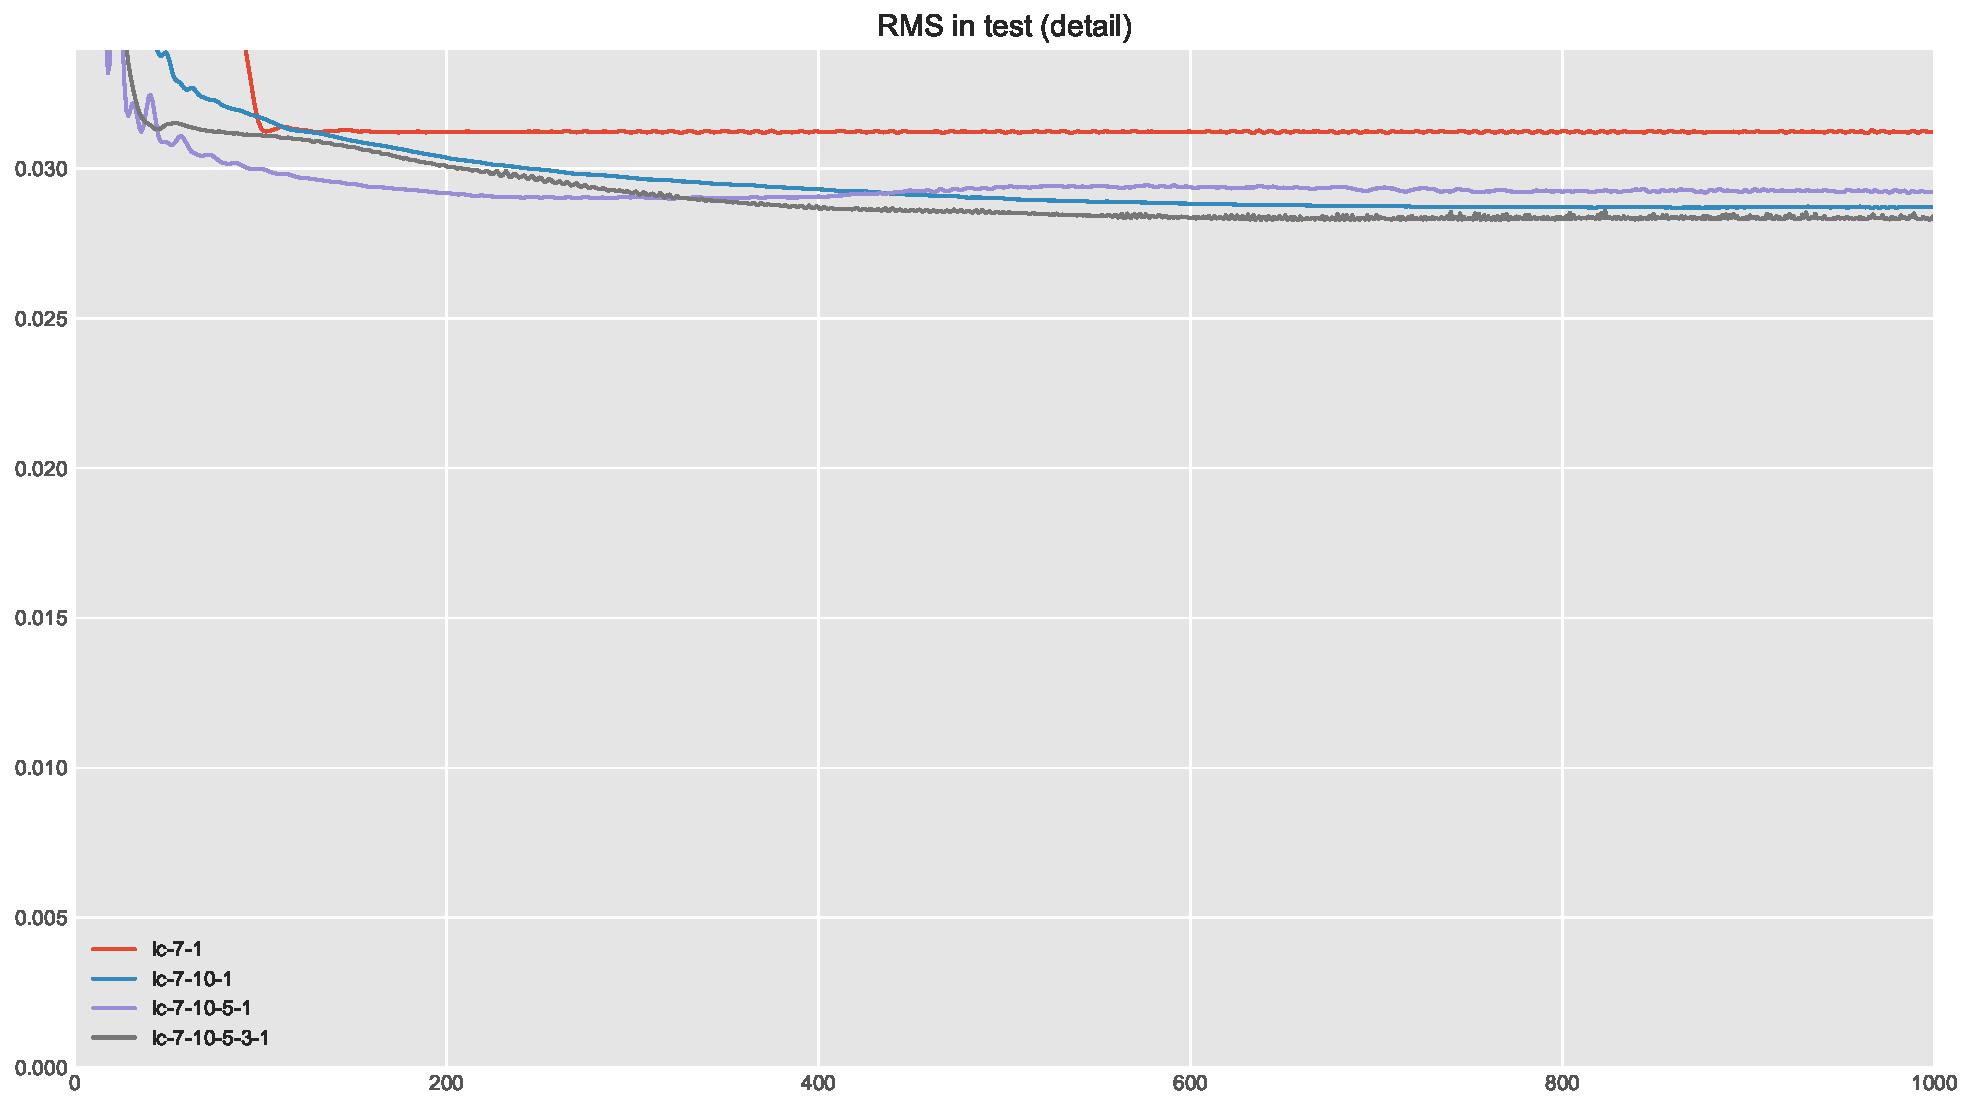
\includegraphics[width=.45\textwidth]{fcs-all-test-detail}}
	\caption[Evolución del error en test de los controladores difusos ajustados]{Visión general y detalle de la evolución del error en test de los diferentes controladores difusos ajustados.}
	\label{fig:adjusted-fcs}
\end{figure}

\TODO{Describir epochs, tiempos de entrenamiento y de inferencia}

\TODO{Separar los entrenamientos para todos los conductores y para los conductores en concreto. En estos últimos, si la red es muy grande, entrenar los modelos tanto desde 0 como desde una red preentrenada.}

\paragraph{Modelo \ac{mlp}}

Para determinar el modelo óptimo de \ac{mlp} en comportamiento longitudinal, se han realizado entrenamientos sobre arquitecturas con diferente cantidad de neuronas y capas ocultas. El resumen de estas arquitecturas se detalla en la tabla~\ref{tbl:cf-mlp-architectures}.

\begin{table}[t]
	\caption[Arquitecturas de \ac{mlp} para el modelo longitudinal]{Resumen de las arquitecturas de \ac{mlp} para el modelo longitudinal. La posición de cada número de la topología indica la capa, siendo su valor el número de nodos (neuronas) que incluye dicha capa.}
	\label{tbl:cf-mlp-architectures}
	\begin{tabular}{ll}
		\toprule
		Nombre & Topología \\
		\midrule
		$MLP_1$ & $7, 1$ \\
		$MLP_2$ & $7, 10, 1$ \\
		$MLP_3$ & $7, 10, 5, 1$ \\
		$MLP_4$ & $7, 10, 5, 3, 1$ \\
		$MLP_5$ & $7, 10, 5, 5, 3, 1$ \\
		\bottomrule
	\end{tabular}
\end{table}

Las arquitecturas han sido entrenadas usando con función de activación \ac{relu} y tangente hiperbólica. 

\TODO{Describir el proceso de entrenamiento del controlador. Poner las grafiquitas de las diferentes arquitecturas usadas y selección de la mejor}

\TODO{Describir epochs, tiempos de entrenamiento y de inferencia.}

\TODO{Separar los entrenamientos para todos los conductores y para los conductores en concreto. En estos últimos, si la red es muy grande, entrenar los modelos tanto desde 0 como desde una red preentrenada.}

\paragraph{Comparación entre modelos}

\TODO{Sacar las gráficas para comparar sus RMS, decir cuál es el mejor e indicar que se usará ese.}